
%(BEGIN_QUESTION)
% Copyright 2006, Tony R. Kuphaldt, released under the Creative Commons Attribution License (v 1.0)
% This means you may do almost anything with this work of mine, so long as you give me proper credit

Study this illustration of a simple pneumatic proportional controller (the beam serves as a baffle, or flapper, for the nozzle to sense):

$$\includegraphics[width=15.5cm]{i01481x01.eps}$$

Answer the following questions about this controller mechanism:

\begin{itemize}
\item{} Is it {\it direct} or {\it reverse} acting?
\vskip 5pt
\item{} What would be required to invert the action of the controller, from direct to reverse action or vice-versa?
\vskip 5pt
\item{} Does it work on the {\it force-balance} or {\it motion-balance} principle?
\vskip 5pt
\item{} How could the setpoint of this controller be adjusted?
\vskip 5pt
\item{} How could the gain (proportional band) of this controller be adjusted?  How about the bias?
\end{itemize}

\vskip 20pt \vbox{\hrule \hbox{\strut \vrule{} {\bf Suggestions for Socratic discussion} \vrule} \hrule}

\begin{itemize}
\item{} The distinction between force-balance and motion-balance is one that tends to confuse students.  A common tactical error students make is to attempt to memorize distinguishing characteristics in order to identify what type of balancing a particular mechanism employs.  A better approach is to {\it think through} the operation of such pneumatic mechanisms using ``thought experiments'' to identify which balance principle they employ.  Why do you think it is bad to go with the memorization approach instead of the ``thought experiment'' approach?
\item{} What difference does it make to us (as technicians) to know whether a mechanism is force- or motion-balance?  In other words, who cares???
\item{} Identify what would need to be modified and/or added to this mechanism to equip it with a {\it manual} mode.
\end{itemize}

\underbar{file i01481}
%(END_QUESTION)





%(BEGIN_ANSWER)

\noindent
{\bf Partial answer:}

\vskip 10pt

\begin{itemize}
\item{} What would be required to invert the action of the controller, from direct to reverse action or vice-versa? {\bf Flip the process variable bellows from the top side of the beam to the bottom side of the beam}.
\vskip 5pt
\item{} How could the setpoint of this controller be adjusted? {\bf Moving the nozzle closer to or further away from the beam}.
\end{itemize}


%(END_ANSWER)





%(BEGIN_NOTES)

\begin{itemize}
\item{} Is it {\it direct} or {\it reverse} acting? {\bf Direct acting}.
\vskip 5pt
\item{} What would be required to invert the action of the controller, from direct to reverse action or vice-versa? {\bf Flip the process variable bellows from the top side of the beam to the bottom side of the beam}.
\vskip 5pt
\item{} Does it work on the {\it force-balance} or {\it motion-balance} principle? {\bf Motion balance}.
\vskip 5pt
\item{} How could the setpoint of this controller be adjusted? {\bf Moving the nozzle closer to or further away from the beam}.
\vskip 5pt
\item{} How could the gain (proportional band) of this controller be adjusted? {\bf Moving the nozzle to the left or to the right}.
\end{itemize}

\vskip 10pt

This controller design is based loosely on the Fisher ``Multi-Trol,'' using the same motion-balance arrangement.

%INDEX% Control, proportional: pneumatic motion-balance controller

%(END_NOTES)


